\documentclass[../competing_bandits.tex]{subfiles}
\begin{document}

\section{Algorithms' Performance in Isolation}\label{section:4}

We start with a pilot experiment in which we investigate each algorithm's performance ``in isolation": in a stand-alone MAB problem without competition. We focus on reputation scores generated by each algorithm.

First, we confirm that\gaedit{, for a sufficiently long time horizon,} algorithms' performance is ordered as we'd expect:
    $\TS \gg \DEG \gg \DG$.
For each algorithm and each MAB instance, we compute the mean reputation score at each round, averaged over all \MRVs. We plot the \emph{mean reputation trajectory}: how this score evolves over time. Figure \ref{prelim_means} shows such \gaedit{a} plot for the Needle In Haystack instance (for other MAB instances the plots are similar). We summarize this finding as follows:

\begin{finding}
\textit{The mean reputation trajectories\gaedit{, for sufficiently long time horizon,} are arranged as predicted by prior work:
    $\TS > \DEG > \DG$.}
\end{finding}


\begin{figure}
\caption{Mean reputation trajectories for Needle-in-Haystack. The shaded area displays 95\% confidence intervals.}
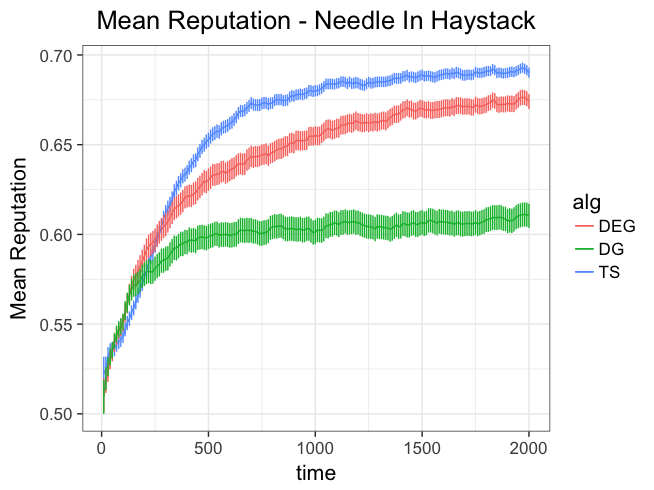
\includegraphics[scale=0.35]{figures/nih_iso_mean}
\label{prelim_means}
%\caption*{\tiny{Mean reputation trajectory The plots contain the average reputation over $1000$ runs for a memory size of $100$ where, for a given $t$, we record the reputation of a given algorithm on a given instance and then average this value across all the runs. The shaded area display 95\% confidence intervals.}}
\end{figure}

The mean reputation trajectory is, arguably, the most natural way to represent an algorithm's performance on a given problem instance. But is it the right statistic for our purposes? That is, how well do these trajectories predict the outcomes of the competition game?

Our experiments led us to consider a statistic with a more direct connection to the competition game: for each time $t$, the proportion of \MRVs for which one algorithm has a higher reputation score than the other which we define as the \textit{relative reputation proportion}.



\begin{figure}[ht]
\caption{Relative Reputation Proportion Plots for $\TS$ vs $\DG$. Shaded area display 95\% confidence intervals.}
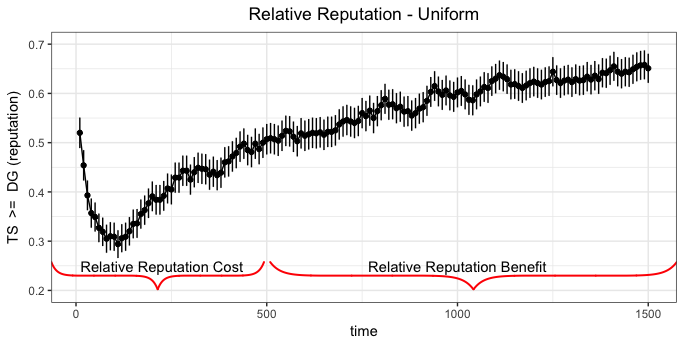
\includegraphics[scale=0.35]{figures/relative_uniform_annotated_plot}
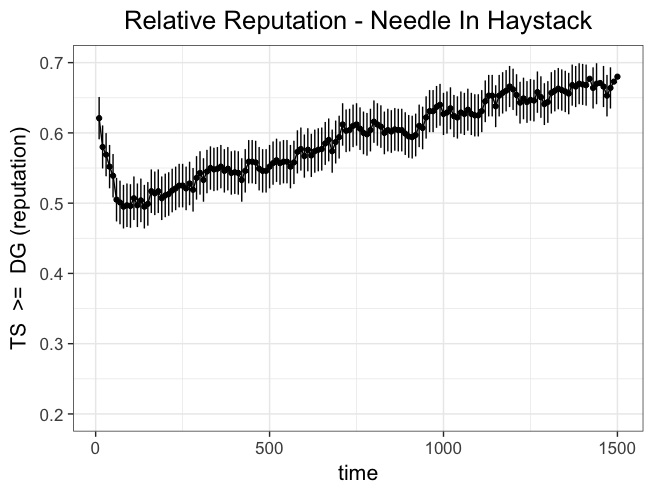
\includegraphics[scale=0.35]{figures/relative_nih_ts_dg.png}
%\caption*{\tiny{The plots contain the average reputation over $1000$ runs for a memory size of $100$ where, for a given $t$, we record the reputation of both of the algorithms on a given instance and then calculate the proportion of runs where $\TS \geq \DG$. The shaded area display 95\% confidence intervals.}}
\label{relative_rep_plots}

\end{figure}

Figure \ref{relative_rep_plots} shows plots of the relative reputation proportion for $\TS$ vs $\DG$ on the Uniform and Needle In Haystack instances. For the Uniform instance we see that, in the early rounds, the relative reputation proportion for $\TS$  vs. $\DG$ is less than 0.5 meaning that $\DG$ has a higher reputation in a majority of the simulations but that, eventually, $\TS$ has a higher reputation than $\DG$ in a majority of the simulations. The intuition behind this is that, especially since the firms start with no substantive initial information, $\TS$ does purposeful exploration in the early rounds in order to acquire information which leads to a relatively lower reputation compared to $\DG$. However, eventually the information acquired from purposeful exploration in the early rounds allows $\TS$ to make better decisions and achieve a higher reputation, especially when the instance is ``hard enough" so that $\DG$ cannot trivially find the best arm.


\begin{definition}
\textit When purposeful exploration leads to a relative reputation loss compared to the greedy alternative we define this as a \textit{relative reputation cost}. The eventual gain in reputation from the early acquired information leads to what we define as a \textit{relative reputation benefit}. Here we treat it as an empirical definition based on the relative reputation proportion where the ``cost" regime is when the proportion $< 0.5$ and the ``benefit" regime is when the proportion is $> 0.5$ for the better algorithm. We call the instances where there is an early costly period followed by a later benefit period \textit{relative reputation costly instances}.
\end{definition}

\begin{finding}
\textit{Purposeful exploration can lead to relative reputational costs and, as a result, the relative reputation proportion of $\TS$ vs $\DG$ favors $\DG$ for small time horizons. We observe this under the Uniform and Heavy Tail instances. However, it is not observed under the Needle In Haystack instances}
\end{finding}

Is exploration always costly? Figure \ref{relative_rep_plots} also shows that for the Needle In Haystack instances, $\TS$ always does relatively better than $\DG$. There are two contributing factors to this. First, $\TS$ identifies the best arm faster in the Needle In Haystack instances than the Uniform instances so that there is a shorter time horizon where $\TS$ needs to engage in purposeful exploration. Second, in the Needle In Haystack instances there are no ``bad" arms as there may be in the Uniform instances since by construction all the arms except one in Needle In Haystack are the same. Thus, when $\TS$ pulls a sub-optimal arm relative to its current information, the expected reward is the same as the greedy option that has not identified the best arm. However, with the Uniform instances, it is possible that the sub-optimal arm that is pulled has substantially lower expected reward relative to the greedy option. Thus, only the Uniform and Heavy Tail instances are relative reputation costly instances.


\OMIT{The following conjecture is natural:

\begin{conjecture}\label{conj:mean-trajectories}
For a given MAB instance, if one algorithm's mean reputation trajectory lies above another at time $T_0$, then the first algorithm prevails in the competition game.
\end{conjecture}

We revisit this conjecture after documenting the results in the competition game.
}

\OMIT{
However, we find a more nuanced picture. 

\begin{finding}
\textit{
Conjecture~\ref{conj:mean-trajectories} is false. Mean reputation trajectories do not suffice to explain the outcomes under competition.}
\end{finding}

We will revisit this finding after presenting the results from the competition game.

\OMIT{ %%%%%
\begin{finding}
\textit{The mean performance of an algorithm is not a sufficient statistic for understanding the performance of an algorithm in competition. Looking at the distribution of reputation difference between algorithms we find that it tend is skewed to the right. Additionally we provide a counterexample where the mean performance does not predict the result of the competition game.}
\end{finding}
} %%%%%

\begin{figure}[H]
\caption{Distribution of reputation scores for Needle-in-Haystack at $t=500$ (smoothed using a kernel density estimate)}
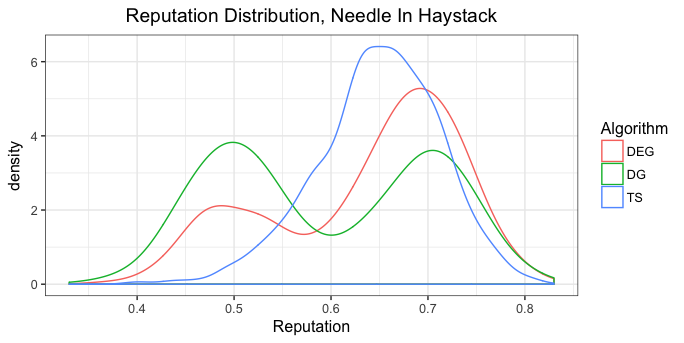
\includegraphics[scale=0.35]{figures/rep_distribution_nih}
\label{rep_dist_nih}
%\caption*{\tiny{The plots contain a kernel density estimate of the reputation distribution at $t = 500$}}
\end{figure}

To see what could go wrong, consider how an algorithm's reputation score is distributed at a particular time. That is, consider the empirical distribution of this score over different \MRVs. For concreteness, we consider the needle-in-haystack instance at time $t=500$ (Figure \ref{rep_dist_nih}).
We see that the ``naive" algorithms $\DG$ and $\DEG$ have a bi-modal reputation distribution, whereas $\TS$ does not. The reason is that for this MAB instance, $\DG$ either finds the best arm and sticks to it, or gets stuck on the bad arms. This leads to two cases: $\DG$ either does slightly better than $\TS$ or where $\TS$ does substantially better than $\DG$.

However, the mean reputation trajectory of an algorithm would summarize all this complexity the average over the \MRVs. This may be inadequate for explaining the outcome of the duopoly game, given that the latter is determined by a simple comparison between the firm's reputation scores. Further, consider the difference in reputation scores (\emph{reputation difference}) between \TS and \DG on a particular \MRV. Let's plot the empirical distribution of the reputation difference (over the \MRVs) at a particular time point. Figure~\ref{ts_dg_rep_diff_nih} shows such plots for several time points. We see that the distribution is skewed to the right, for which the mean is not a representative statistic.  \ascomment{so what?}


\OMIT{ %%%%%%%%
 or not. If it does, then since it engages in no purposeful exploration it will do better than any algorithm that engages in purposeful exploration over sufficiently many rounds. However, if it does not then it will get stuck on a bad arm and lose to $\TS$ or $\DEG$. In these cases its reputation may be substantially worse but for the competition game the relative comparison between them is all that matters \footnote{This holds for our model and the decision rule of the agents, though the absolute difference may matter if, for instance, we consider the SoftMax decision rule in \cite{CompetingBandits-itcs16}}.
} %%%%%%%%


\OMIT{There are alternative statistics that we could consider such as the median or numerically calculating $\Pr(reputation(\TS) - reputation(\DG)) > 0$ using the estimated density, but instead we define a simple and natural statistic to help us reason about what happens under competition, the \textit{relative reputation proportion}.} 

\begin{figure}[H]
\caption{Distribution of reputation difference $\TS-\DG$ for the Needle-in-Haystack (smoothed via a kernel density estimate)}
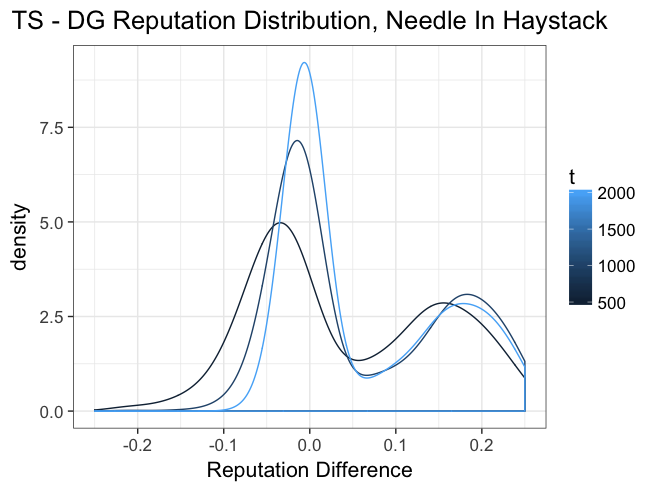
\includegraphics[scale=0.35]{figures/ts_dg_rep_diff_nih}
\label{ts_dg_rep_diff_nih}
%\caption*{\tiny{The plots contain a kernel density estimate of the difference in reputation between $\TS$ and $\DG$ across $t$}}
\end{figure}

. 

\ascomment{Stopped here.}

\begin{definition}
\textit{Relative Reputation Proportion} - the proportion of simulations in which algorithm $A$ had at least as high of a reputation as algorithm $B$ for a fixed time $t$
\end{definition}


\begin{finding}
\textit{Purposeful exploration can lead to relative reputational costs compared to the greedy alternative and this leads to $\TS$ doing worse than $\DG$ for small time horizons. We observe this under the Uniform and Heavy Tail priors. However, it is not observed under the Needle In Haystack prior}
\end{finding}

The relative reputation statistic corresponds to running the bandit algorithms in isolation on the same instance and with the same realizations for $t$ rounds and then calculating the fraction of simulations at which an agent would select a firm playing $A$ over a firm playing $B$ at time $t$ \footnote{As further motivation for this statistic, one may be interested in if there is ever a case where, for sufficiently large $t$, we observe that $\DEG >\DG$ or $\TS > \DG$ according to the mean reputation but $\DG > \DEG$ or $\DG > TS$ according to the relative reputation proportion. In the supplementary material we have results showing that, for Heavy Tail prior with $K=3$ we have that $\DEG > \DG$ according to the mean reputation but $\DG > \DEG$ according to the relative reputation proportion. Additionally, these results carry over to the competition game}.

\begin{figure}[ht]
\caption{Relative Reputation Plots}
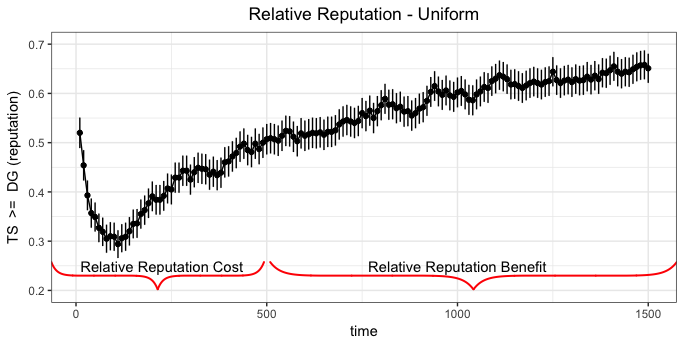
\includegraphics[scale=0.35]{figures/relative_uniform_annotated_plot}
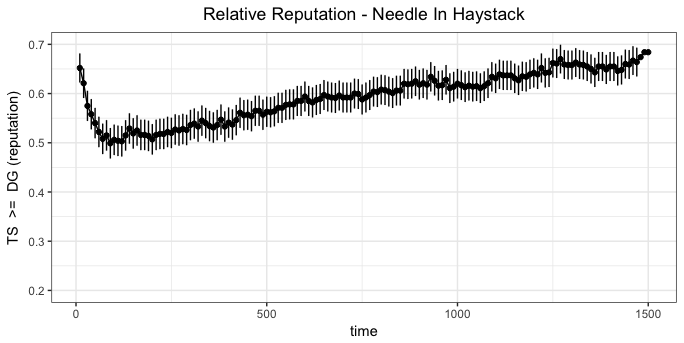
\includegraphics[scale=0.35]{figures/ts_dg_nih_10_prelim}
\caption*{\tiny{The plots contain the average reputation over $1000$ runs for a memory size of $100$ where, for a given $t$, we record the reputation of both of the algorithms on a given instance and then calculate the proportion of runs where $\TS \geq \DG$. The shaded area display 95\% confidence intervals.}}
\label{relative_rep_plots}

\end{figure}



Figure \ref{relative_rep_plots} shows plots of the relative reputation proportion for $\TS$ vs $\DG$ on the Uniform and Needle In Haystack prior. For the Uniform prior we see that, in the early rounds, $\DG > \TS$ for the majority of the simulations but that, eventually, $\TS > \DG$. The intuition behind this is that, especially since the firms start with no substantive initial information, $\TS$ does purposeful exploration in the early rounds in order to acquire information. However, eventually the information acquired from purposeful exploration in the early rounds allows $\TS$ to make better decisions and achieve a higher reputation, especially when the instance is ``hard enough" so that $\DG$ cannot trivially find the best arm. The early exploration leads to what we define as a \textit{relative reputation cost} and the eventual gain in reputation leads to what we define as a \textit{relative reputation benefit}.



\begin{definition}
\textit{Relative reputation cost and benefit} - the relative reputation loss an algorithm incurs from purposeful exploration compared to the greedy alternative. Here we treat it as an empirical definition based on the relative reputation proportion where the ``cost" regime is when the proportion $< 0.5$ and the ``benefit" regime is when the proportion is $> 0.5$ for the better algorithm. We call the priors where there is an early costly period followed by a later benefit period relative reputation costly priors.
\end{definition}
Is exploration always costly? Figure \ref{relative_rep_plots} also shows that for the Needle In Haystack prior, $\TS$ always does relatively better than $\DG$. There are two contributing factors to this. First, $\TS$ identifies the best arm faster in the Needle In Haystack prior than the Uniform prior so that there is a shorter time horizon where $\TS$ needs to engage in purposeful exploration. Second, in the Needle In Haystack prior there are no ``bad" arms as there may be in the Uniform prior since by construction all the arms except one in Needle In Haystack are the same. Thus, when $\TS$ pulls a sub-optimal arm relative to its current information, the expected reward is the same as the greedy option that has not identified the best arm. However, with the Uniform prior, it is possible that the sub-optimal arm that is pulled has substantially lower expected reward relative to the greedy option. Thus, only the Uniform and Heavy Tail priors are relative reputation costly priors.

}

\end{document} 